\documentclass{article}
\usepackage{blindtext}
\usepackage{graphicx}
\usepackage[T1]{fontenc}
\usepackage[utf8]{inputenc} 
\usepackage[margin = 0.75in]{geometry}
\usepackage{amsmath}
\usepackage{systeme}
\usepackage{hyperref}

\begin{document}
 \section*{\LARGE{Exchange and Correlation holes}}
 \vspace{0.5cm}
 \subsection*{\Large{Density Matrix}}
 \begin{Large}
 \begin{flushleft}
 If we want to see whether an exchange-correlation functional should work or not, we should look at how well it describes the exchange-correlation hole. To understand what the previous line means, lets start by defining a \textbf{first order density matrix} as follows:
  \begin{equation}\label{eq:1}
  \gamma(\textbf{x},\textbf{x'}) = N \displaystyle{\int}d\textbf{x}_2d\textbf{x}_3...d\textbf{x}_N\Psi^*(\textbf{x},\textbf{x}_2,\textbf{x}_3,...,\textbf{x}_N)\Psi(\textbf{x'},\textbf{x}_2,\textbf{x}_3,...,\textbf{x}_N)
  \end{equation}
  Note that in eqn(\ref{eq:1}), in $\Psi^*$, the $e^-_1$ is at \textbf{x}, while in $\Psi$, $e^-_1$ is at \textbf{x'}. If we take the Kohn-Sham wavefunction as a single determinant\footnote{All the derivations from now onwards are done by takin single determinants only. The same derivation can be done even if we have a linear combination of many determinants.} 
  \begin{equation}\label{eq:2}
  \begin{split}
  \Psi_{ks}(\textbf{x}_1,\textbf{x}_2,...,\textbf{x}_N) &= 
  \begin{vmatrix}
  \phi_i(\textbf{x}_1) & \phi_j(\textbf{x}_1) & ... & \phi_k(\textbf{x}_1)\\
  \phi_i(\textbf{x}_2) & \phi_j(\textbf{x}_2) & ... & \phi_k(\textbf{x}_2)\\
  \vdots & \vdots & \ddots & \vdots\\
  \phi_i(\textbf{x}_N) & \phi_j(\textbf{x}_N) & ... & \phi_k(\textbf{x}_N)\\
  \end{vmatrix}\\
  &= \frac{1}{\sqrt{N!}}\sum_{n=1}^{N!}(-1)^{p_n}P_n[\phi(\textbf{x}_1)\phi(\textbf{x}_2)...\phi(\textbf{x}_N)] 
  \end{split}
  \end{equation}
  Using eqn(\ref{eq:2}) we can get a first-ordr density matrix for the single-determinant Kohn-Sham wavefunction via eqn(\ref{eq:1}) as follows,
  \begin{equation}\label{eq:3}
  \begin{split}
  \gamma_{ks}(\textbf{x},\textbf{x'}) = &\frac{N}{N!}\sum_{n=1}^{N!}\sum_{m=1}^{N!}(-1)^{p_n}(-1)^{p_m}\displaystyle{\int}d\textbf{x}_2...d\textbf{x}_N P_n[\phi_i^*(\textbf{x})\phi_j^*(\textbf{x}_2)...\phi_k^*(\textbf{x}_N)]\times\\&\,\,\,\,\,\,\,\,\,\,\,\,\,\,\,\,\,\,\,\,\,\,\,\,\,\,\,\,\,\,P_m[\phi_i(\textbf{x'})\phi_j(\textbf{x}_2)...\phi_k(\textbf{x}_N)] 
  \end{split}  
  \end{equation}
  The integral is of all variables from $\textbf{x}_2$ to $\textbf{x}_N$. Here, since all the Kohn-Sham spin-orbitals $\phi_i(\textbf{x})$ are orthonormal, only permutations where the $e^-_2$ to $e^-_N$ are occupying the same $\phi_i(\textbf{x})$ in both the permutations will survive. So we have
  \begin{equation}\label{eq:4}
  \begin{split}
  \gamma_{ks}(\textbf{x},\textbf{x'}) = &\frac{1}{(N-1)!}\sum_{n=1}^{N!}\displaystyle{\int}d\textbf{x}_2...d\textbf{x}_N P_n[\phi_i^*(\textbf{x})\phi_j^*(\textbf{x}_2)...\phi_k^*(\textbf{x}_N)]\times\\&\,\,\,\,\,\,\,\,\,\,\,\,\,\,\,\,\,\,\,\,\,\,\,\,\,\,\,\,\,\,\,\,\,\,\,\,\,P_n[\phi_i(\textbf{x'})\phi_j(\textbf{x}_2)...\phi_k(\textbf{x}_N)] 
  \end{split}
  \end{equation} 
  We can think of the summation over all the $N!$ permutations as $\rightarrow$ $e^-_1$ can occupy any one of the $N$ kohn-sham single particle spin-orbitals $\phi_i(\textbf{x})$. For each such occupation, the remaining $(N-1)$ $e^-$ can rearrange themselves in the remaining $(N-1)$ spin orbitals in $(N-1)!$ ways. Thus eqn(\ref{eq:4}) becomes,
  \begin{equation}\label{eq:5}
  \gamma_{ks}(\textbf{x},\textbf{x'}) = \frac{(N-1)!}{(N-1)!}\sum_n^N\phi_n^*(\textbf{x})\phi_n(\textbf{x'})
  \end{equation}
  or
  \begin{equation}\label{eq:6}
  \gamma_{ks}(\textbf{x},\textbf{x'}) = \sum_n^N\phi_n^*(\textbf{x})\phi_n(\textbf{x'})
  \end{equation}
  So we can see that the diagonal elements (\textbf{x}=\textbf{x'}) will just give the $e^-$ densities
  \begin{equation}\label{eq:7}
  \begin{split}
  \gamma_{ks}(\textbf{x},\textbf{x}) &= \sum_n^N\phi_n^*(\textbf{x})\phi_n(\textbf{x}) = \sum_n^N|\phi_n^*(\textbf{x})|^2\\
  &= \rho(\textbf{x})
  \end{split}
  \end{equation}
 \end{flushleft}
 \end{Large} 
  
 \subsection*{\Large{Pair Density}}
 \begin{Large}
  \begin{flushleft}
  We will now define a quantity called \textbf{Pair Density} as
  \begin{equation}\label{eq:8}
  P(\textbf{x},\textbf{x'}) = N(N-1)\displaystyle{\int}d\textbf{x}_3...d\textbf{x}_N|\Psi(\textbf{x},\textbf{x'},\textbf{x}_3,...,\textbf{x}_N)|^2
  \end{equation}
  We can think of the Pair density as 
  \begin{equation}\label{eq:9}
  \begin{split}
  P(\textbf{x},\textbf{x'})\,d\textbf{x}\,d\textbf{x'} &= \rho(\textbf{x})\rho_2(\textbf{x};\textbf{x'})d\textbf{x}\,d\textbf{x'}\\
  &= \left\lbrace \rho(\textbf{x})d\textbf{x}\right\rbrace \left\lbrace \rho_2(\textbf{x};\textbf{x'})d\textbf{x'}\right\rbrace
  \end{split}
  \end{equation}
  where $n_2(\textbf{x};\textbf{x'})d\textbf{x'}$ is the conditional probability of finding a $e^-_2$ at $d\textbf{x'}$ of \textbf{x'} given $e^-_1$ is at $d\textbf{x}$ of \textbf{x}. So $P(\textbf{x},\textbf{x'})$ is the probability of obtaining an indistinct pair of $e^-$ simultaneously at two points in space.
  
  \subsubsection*{\Large{Density from Pair-density}}
  Integrating eqn(\ref{eq:8}) with respect to \textbf{x'},
  \begin{equation}\label{eq:10}
  \displaystyle{\int}P(\textbf{x},\textbf{x'})\,d\textbf{x'} = N(N-1)\displaystyle{\int}d\textbf{x'}d\textbf{x}_3...d\textbf{x}_N|\Psi(\textbf{x},\textbf{x'},\textbf{x}_3,...,\textbf{x}_N)|^2
  \end{equation}
  Rearranging the equation and replacing the dummy variable \textbf{x'} with dummy variable $\textbf{x}_2$ we see that,
  \begin{equation}\label{eq:11}
  \displaystyle{\int}P(\textbf{x},\textbf{x}_2)\,d\textbf{x}_2 = (N-1)\left(N\displaystyle{\int}d\textbf{x}_2d\textbf{x}_3...d\textbf{x}_N|\Psi(\textbf{x},\textbf{x}_2,\textbf{x}_3,...,\textbf{x}_N)|^2\right)
  \end{equation} 
  Looking closely at eqn(\ref{eq:11}) and comparing with eqn(\ref{eq:1}), we realise that the term inside parenthesis is just the diagonal element of the first order density matrix. So from eqn(\ref{eq:7}) we have,
  \begin{equation}\label{eq:12}
  \displaystyle{\int}P(\textbf{x},\textbf{x'})\,d\textbf{x'} = (N-1)\rho(\textbf{x})
  \end{equation} 
  So as we can see from eqn(\ref{eq:12}) that knowing the ground-state pair-density of a system can give us the ground-state denisty of that system. Thus using the Hohenberg-Kohn theorem we can say that the Pair-density can in-principle determine all the ground-state properties of a system.
  
  \subsubsection*{\Large{Self-interaction error via pair-density}}   
  Lets see what happens if $\rho_2(\textbf{x};\textbf{x'})=\rho(\textbf{x'})$ i.e. in the case of independent particles,
  \begin{equation}\label{eq:13}
  \begin{split}
  \displaystyle{\int}P(\textbf{x},\textbf{x'})d\textbf{x'} &= \rho(\textbf{x})\displaystyle{\int}\rho(\textbf{x'})d\textbf{x'}\\
  &= N\rho(\textbf{x})
  \end{split}
  \end{equation}
  Here we can easily see by comparing with eqn(\ref{eq:12}), that \textbf{eqn(\ref{eq:13}) is wrong} by definition.This discrepancy arises as we have an extra interaction of an $e^-$ with itself which gives rise to one extra pair than should be the case. This error is often called the \textbf{Self-interaction error}. So we can conclude from eqn(\ref{eq:12}) and eqn(\ref{eq:13}) that 
  \begin{equation}\label{eq:14}
  \rho_2(\textbf{x};\textbf{x'}) < \rho(\textbf{x'})
  \end{equation}
  Eqn(\ref{eq:14}) should be obeyed so that eqn(\ref{eq:12}) is followed. So we see that the pair-density helps us understand that the independent particle model will fail to identify the number of indistinct electron pair in an interacting system. 
  
 \subsubsection*{\Large{$V_{ee}^{gs}$ from Pair-density}}  
  Since we can determine the $\rho_{gs}$ we can in-principle also calculate the ground-state potential energy due the $e^--e^-$ interaction of an $Ne^-$ system if we know the pair-density. We now try to determine the functional form of $V_{ee}$ in terms of $P(\textbf{x},\textbf{x'})$,
  \begin{equation}\label{eq:15}
  V_{ee}^{gs} =\left\langle\Psi_{gs}(\textbf{x}_1,\textbf{x}_2,...\textbf{x}_N)\Bigg|\sum_{i=1}^N\sum_{j>i}^N\frac{1}{|\textbf{r}_i-\textbf{r}_j|}\Bigg|\Psi_{gs}(\textbf{x}_1,\textbf{x}_2,...\textbf{x}_N)\right\rangle
  \end{equation}
  Since all the $e^-$ are identical, the above sum is just the sum over all the distinct pair of $e^-$. So we can write,
  \begin{equation}\label{eq:16}
 V_{ee}^{gs} = \frac{N(N-1)}{2}\left\langle\Psi_{gs}(\textbf{x}_1,\textbf{x}_2,...\textbf{x}_N)\Bigg|\frac{1}{|\textbf{r}_1-\textbf{r}_2|}\Bigg|\Psi_{gs}(\textbf{x}_1,\textbf{x}_2,...\textbf{x}_N)\right\rangle
  \end{equation}
  We can now exapand this integral as,
  \begin{equation}\label{eq:17}
  V_{ee}^{gs} = \frac{N(N-1)}{2}\displaystyle{\iint}\frac{d\textbf{x}_1\textbf{x}_2}{|\textbf{r}_1-\textbf{r}_2|}\left(\displaystyle{\int}|\Psi_{gs}(\textbf{x}_1,\textbf{x}_2,...\textbf{x}_N)|^2d\textbf{x}_3...d\textbf{x}_N\right)
  \end{equation}
  Comparing eqn(\ref{eq:15}) with eqn(\ref{eq:8}) we can rewrite eqn(\ref{eq:12}) as,
  \begin{equation}\label{eq:18}
  V_{ee}^{gs}[P(\textbf{x}_1,\textbf{x}_2)] = \frac{1}{2}\displaystyle{\iint}\frac{P(\textbf{x}_1,\textbf{x}_2)}{|\textbf{r}_1-\textbf{r}_2|}d\textbf{x}_1\textbf{x}_2
  \end{equation}
  \end{flushleft}
 \end{Large}
 
 \subsection*{\Large{Holes}}
  \begin{Large}
   \begin{flushleft}
    From the above section we now know that we can obtain many information about the system if we can somehow obtain the $P(\textbf{x}_1,\textbf{x}_2)$. So to get some information about $P(\textbf{x}_1,\textbf{x}_2)$, we now do the following,
    \begin{equation}\label{eq:19}
    P(\textbf{x}_1,\textbf{x}_2) = \rho(\textbf{x}_1)[\rho(\textbf{x}_2)+\rho_{xc}(\textbf{x}_1,\textbf{x}_2)]
    \end{equation}
    So we have now divided the $P(\textbf{x}_1,\textbf{x}_2)$ into a non-interacting part and an $\rho_{xc}$ part which will correct the self-interactions in the non-interacting part i.e. $\rho_{xc}$ will try to remove the extra $e^-$ present in the first term and hence $\rho_{xc}$ is called the \textbf{exchange-correlation hole}. Putting eqn(\ref{eq:19}) in eqn(\ref{eq:18}) we have,
    \begin{equation}\label{eq:20}
    \begin{split}
    V_{ee}^{gs} &= \frac{1}{2}\displaystyle{\iint}\frac{\rho(\textbf{x}_1)[\rho(\textbf{x}_2)+\rho_{xc}(\textbf{x}_1,\textbf{x}_2)]}{|\textbf{r}_1-\textbf{r}_2|}d\textbf{x}_1\textbf{x}_2\\
    &= \frac{1}{2}\displaystyle{\iint}\frac{\rho(\textbf{x}_1)\rho(\textbf{x}_2)}{|\textbf{r}_1-\textbf{r}_2|}d\textbf{x}_1\textbf{x}_2 + \frac{1}{2}\displaystyle{\iint}\frac{\rho(\textbf{x}_1)\rho_{xc}(\textbf{x}_1,\textbf{x}_2)}{|\textbf{r}_1-\textbf{r}_2|}d\textbf{x}_1\textbf{x}_2
    \end{split}
    \end{equation}
    We can immediately recognise that the first term is the Classical-Coulomb interaction between the $e^-$ densities. So, we rewrite eqn(\ref{eq:18}) as,
    \begin{equation}\label{eq:21}
    V_{ee}^{gs} = U_{Hartree}[\rho] + E_{xc}[\rho]
    \end{equation} 
    where,
    \begin{equation}\label{eq:22}
    U_{Hartree}[\rho] = \frac{1}{2}\displaystyle{\iint}\frac{\rho(\textbf{x}_1)\rho(\textbf{x}_2)}{|\textbf{r}_1-\textbf{r}_2|}d\textbf{x}_1\textbf{x}_2
    \end{equation}
    is the Classical-Coulomb or the Hartree energy and
    \begin{equation}\label{eq:23}
    E_{xc}[\rho] = \frac{1}{2}\displaystyle{\iint}\frac{\rho(\textbf{x}_1)\rho_{xc}(\textbf{x}_1,\textbf{x}_2)}{|\textbf{r}_1-\textbf{r}_2|}d\textbf{x}_1\textbf{x}_2
	\end{equation}
	is called the Exchange-Correlation energy\footnote{There is a kinetic contribution also which smoothly connects with eqn(\ref{eq:23}) via adiabatic connection and thus we ignore that here.}.             
   \end{flushleft}
  \end{Large}
  
 \subsection*{\Large{Properties of Exchange-Correlation Hole}}
  \begin{Large}
   \begin{flushleft}
    Eqn(\ref{eq:23}) looks like the $e^-$ density at $\textbf{x}_1$ is interacting with the hole $\rho_{xc}(\textbf{x}_1,\textbf{x}_2)$. Since the $\rho_{xc}(\textbf{x}_1,\textbf{x}_2)$ describes the reduced $e^-$ density around the $e^-$ at $\textbf{x}_1$, we can interpret the second term in eqn(\ref{eq:20}) to be the electrostatic attraction between an $e^-$ and the hole surrounding it. So it is eqn(\ref{eq:23}) which plays the major role in determining how well exchange-correlation energy is, as it's this term which is going to make corrections to the classical contibution. From eqn(\ref{eq:23}), the better we describe the holes $\rightarrow$ the better we approximate the $E_{xc}$. So now lets look at what are the properties of the exact xc-hole.
   \subsubsection*{\Large{Property 1: Sum Rule}}
    Integrating eqn(\ref{eq:19}) with respect to $\textbf{x}_2$ we get,
    \begin{equation}\label{eq:24}
    \displaystyle{\int}P(\textbf{x}_1,\textbf{x}_2)d\textbf{x}_2 = \rho(\textbf{x}_1)\displaystyle{\int}\rho(\textbf{x}_2)d\textbf{x}_2+\rho(\textbf{x}_1)\displaystyle{\int}\rho_{xc}(\textbf{x}_1,\textbf{x}_2)d\textbf{x}_2
    \end{equation}
    From eqn(\ref{eq:12}) we have,
    \begin{equation}\label{eq:25}
    (N-1)\rho(\textbf{x}_1) = N\rho(\textbf{x}_1) + \rho(\textbf{x}_1)\displaystyle{\int}\rho_{xc}(\textbf{x}_1,\textbf{x}_2)d\textbf{x}_2
    \end{equation}
    Rearranging, we get,
    \begin{equation}\label{eq:26}
    \displaystyle{\int}\rho_{xc}(\textbf{x}_1,\textbf{x}_2)d\textbf{x}_2 = -1
    \end{equation}
    Eqn(\ref{eq:26}) signifies that for any $e^-$ in a density, there is exactly one $e^-$ missing from its surrounding i.e. there is an \textbf{hole}, an area of reduced $e^-$ density in its surrounding. Eqn(26) is called the \textbf{Sum rule} and we imagine it like$\rightarrow$ when an $e^-$ is moving through a density it carries with itself a hole.
    
    \subsubsection*{\Large{Property 2: The XC-hole is always negative}}
    By definition, from eqn(\ref{eq:19}) we see that the XC-hole is always negative i.e.
    \begin{equation}\label{eq:27}
    \rho_{xc}(\textbf{x}_1,\textbf{x}_2) < 0
    \end{equation}
    which means there is always an area of reduced $e^-$ density around an $e^-$.
    
    \subsubsection*{\Large{Property 3: There is a finite probability of finding $e^-_2$}}
    As $P(\textbf{x}_1,\textbf{x}_2) > 0$, so
    \begin{equation}\label{eq:28}
    \rho_{xc}(\textbf{x}_1,\textbf{x}_2) > -\rho(\textbf{x}_2)
    \end{equation} 
    This will become clear later (with the $\rho_{xc}$ plot, Point-5 in section-1.5)  
    \subsubsection*{\Large{Property 4: the XC-hole is spherically asymmetric}}
    Since the XC-hole represents a reduction in $e^-$ density, it is often factorised as,
    \begin{equation}\label{eq:29}
    \rho_{xc}(\textbf{x}_1,\textbf{x}_2) = \rho(\textbf{x}_2)f_{xc}(\textbf{x}_1,\textbf{x}_2)
    \end{equation}
    where $f_{xc}$ is just a negative fraction ($-1 < f_{xc}< 0$). This is just another way of saying that the $e^-$ density is reduced when conpared to the independent-particle model. $f_{xc}$ is called the \textbf{Pair-correlation factor}. Now if we look at eqn(\ref{eq:29}), we see that the hole depends on the density at $\textbf{x}_2$ and thus it will vary for different $x_2$, as in general the $e^-$ density of real systems are inhomogeous. Thus the actual XC-hole has angular dependence $\rightarrow$ spherically asymmetric.
    
    \subsubsection*{\Large{Property 5: Property 4 might not be required as a MUST condition}}
    If we look closely at eqn(\ref{eq:23}), we will see that any angular dependence is averaged out, as the integral in eqn(\ref{eq:23}) is due to coulombic interaction which only has dependence on $|\textbf{r}_1-\textbf{r}_2|$, thus any angular dependence will be integrated and thus we only require the properties of the spherically averaged XC-hole.
   \end{flushleft}
  \end{Large}
  
 \subsection*{\Large{How to imagine an XC-hole}}
  \begin{figure}[h]
  \centering
  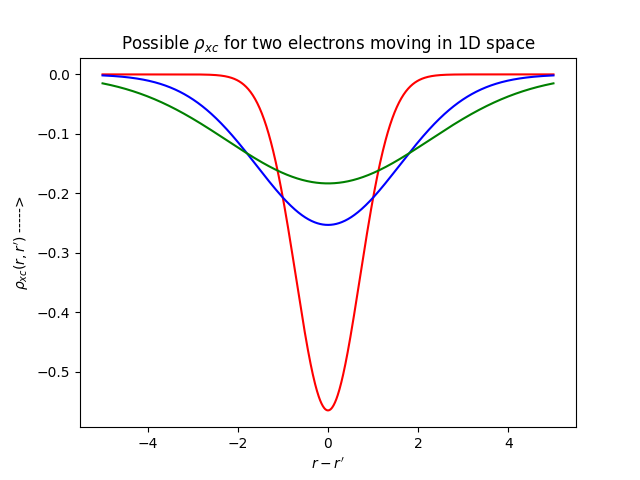
\includegraphics[scale=0.88]{nxc.png}
  \caption{Three different possible $\rho_{xc}$ for two $e^-$ moving in 1D line}
  \label{fig:Hole}
  \end{figure}
  
  \begin{Large}
   \begin{flushleft}
   The above figure is done by taking gaussian functions(subjected to the sum-rule (eqn(\ref{eq:26}))) just to give an idea of how a hole should behave by taking into consideration all the above derivations and properties. It may not be the XC-hole of any system. We should note the following behaviour of an XC-hole from fig(\ref{fig:Hole}),
   \begin{enumerate}
   \item[1]{The hole is always negative.}
   \item[2]{The hole is the most negative when the two $e^-$ are very close each other\footnote{This is often called \textit{Dynamic correlation}. The hole may be the shifted to the nuclear region (i.e. the on-top region of hole is now centered on nucleus) in cases like when a molecule breaks and the atoms move far apart $\rightarrow$ \textit{Static-correlation}. But just for a beginner, the case of \textit{dynamic-correlation} gives a better intuition and we thus stick with that here. For a better discussion, consider chapter-2 of A Chemist’s Guide to
Density Functional Theory, Wolfram Koch, Max C. Holthausen.}}
   \item[3]{The strength of the hole decreases when the two $e^-$ move apart.}
   \item[4]{The spread of the hole increases (i.e. the hole stretches) as the strength of on-top hole (the value of hole at $|\textbf{r}_1-\textbf{r}_2|=0$) decreases and \textit{vice-versa}.}
   \item[5]{Due to point(4), we see that in the limiting case of very strong on-top hole, the curve will approach $-\delta(\textbf{r}_1-\textbf{r}_2)$ behaviour. This cannot happen as it would imply that $e^-_1$ interacts with $e^-_2$ only when $\textbf{r}_1=\textbf{r}_2$, and for all other distances the hole is 0 and then from eqn(\ref{eq:19}) the particles behave as independent particle. But we know that there is clearly a 1/$r_{12}$ coulombic dependence, so $e^-$ are interacting for distances other than $|\textbf{r}_1-\textbf{r}_2|=0$ also. Hence, there should be a strict > inequality in eqn(\ref{eq:28})(Property3) $\rightarrow$ $P(\textbf{x}_1,\textbf{x}_2) > 0$, i.e there should be finite probability of getting two electrons very close. This is actually the case and this gives rise to the $e^-$-$e^-$ cusp condition in the many-$e^-$ wave function to prevent the $e^-$-$e^-$ potential energy from diverging at $r_{12}=0$.}
   \end{enumerate}
   \end{flushleft}
  \end{Large}
  
 \subsection*{\Large{Parts of an XC-hole}}
  \begin{Large}
   \begin{flushleft}
    To understand the nature of the XC-hole, its usually divided in two parts
    \begin{equation}\label{eq:30}
     \rho_{xc}(\textbf{x}_1,\textbf{x}_2) = \rho_{x}(\textbf{x}_1,\textbf{x}_2) + \rho_{c}(\textbf{x}_1,\textbf{x}_2)
    \end{equation}
    where
    \begin{enumerate}
    \item{$\rho_{x}(\textbf{x}_1,\textbf{x}_2)\rightarrow$ The \textbf{exchange(or Fermi)hole} and it arises due to the antisymmetric nature of the many-$e^-$ wavefunction which causes \textit{Pauli-repulsion}. The $\rho_{x}(\textbf{x}_1,\textbf{x}_2)$ is also responsible for the correction to the self-interaction.}
    \item{$\rho_{c}(\textbf{x}_1,\textbf{x}_2)\rightarrow$ The \textbf{Correlation(or Coulomb)hole}}. It arises mainly due to the 1/$r_{12}$ nature of the coulombic interaction and is also responsible for the $e^-$-$e^-$ cusp-condition in the many-$e^-$ wavefunction.
    \end{enumerate}
   \subsubsection*{\Large{Exchange (Fermi) Hole}}
   The exchange-interaction arises whenever we try to use a many-$e^-$ anti-symmetric wavefunction to evaluate the Pair-density (eqn(\ref{eq:8})). Let's evaluate the Pair-density using Kohn-Sham single determinant as our many-$e^-$ antisymmetric wavefunction. Putting eqn(\ref{eq:2}) in eqn(\ref{eq:8}), we get,
   \begin{equation}\label{eq:31}
  \begin{split}
  P_{ks}(\textbf{x}_1,\textbf{x}_2) = &\frac{N(N-1)}{N!}\sum_{n=1}^{N!}\sum_{m=1}^{N!}(-1)^{p_n}(-1)^{p_m}\displaystyle{\int}d\textbf{x}_3...d\textbf{x}_N P_n[\phi_i^*(\textbf{x}_1)\phi_j^*(\textbf{x}_2)...\phi_k^*(\textbf{x}_N)]\times\\&\hspace{6cm}P_m[\phi_i(\textbf{x}_1)\phi_j(\textbf{x}_2)...\phi_k(\textbf{x}_N)] 
  \end{split}  
  \end{equation}
  Now since $\textbf{x}_1$ and $\textbf{x}_2$ are not integrated upon, \textbf{if} 
  \begin{equation}\label{eq:32}
   P_n[\phi^*_i(\textbf{x}_1)\phi^*_j(\textbf{x}_2)...\phi^*_k(\textbf{x}_N)] = \phi^*_i(\textbf{x}_1)\phi^*_j(\textbf{x}_2)...\phi^*_k(\textbf{x}_N)
  \end{equation}
  \textbf{then} we have two possibilities for $P_m$, 
  \begin{equation}\label{eq:33}
  P_m[\phi_i(\textbf{x}_1)\phi_j(\textbf{x}_2)...\phi_k(\textbf{x}_N)] = 
  \left\{
  \begin{array}{rcrcrc@{\qquad}l}
  \phi_i(\textbf{x}_1)\phi_j(\textbf{x}_2)...\phi_k(\textbf{x}_N) \\
  -\phi_i(\textbf{x}_2)\phi_j(\textbf{x}_1)...\phi_k(\textbf{x}_N)\\
  \end{array}
  \right.
  \end{equation}     
  So eq(\ref{eq:31}) now becomes,
  \begin{equation}\label{eq:34}
  \begin{split}
  P_{ks}(\textbf{x}_1,\textbf{x}_2) = &\frac{1}{(N-2)!}\sum_{n=1}^{N!}\displaystyle{\int}d\textbf{x}_3...d\textbf{x}_N P_n[\phi_i^*(\textbf{x}_1)\phi_j^*(\textbf{x}_2)...\phi_k^*(\textbf{x}_N)]\times\\&\hspace{3cm}(1- \mathcal{P}_{12})P_m[\phi_i(\textbf{x}_1)\phi_j(\textbf{x}_2)...\phi_k(\textbf{x}_N)] 
  \end{split}
  \end{equation}
  where $\mathcal{P}_{12}$ exchanges the coordinates of $e^-_1$ and $e^-_2$. The integral is of all variables from $\textbf{x}_3$ to $\textbf{x}_N$. So for any two $\phi_i$ occupied by $\textbf{x}_1$ and $\textbf{x}_2$,the remaining $(N-2)e^-$ can occupy the remaining $(N-2)\phi_i$ in $(N-2)!$ ways. Also, since all the Kohn-Sham spin-orbitals $\phi(\textbf{x})$ are orthonormal, only permutations in which $e^-_3$ to $e^-_N$ are occupying the same $\phi_i(\textbf{x}_i)$ in both $P_n$ and $P_m$ will survive. So we have
  \begin{equation}\label{eq:35}
  \begin{split}
  P_{ks}(\textbf{x}_1,\textbf{x}_2) &= \frac{(N-2)!}{(N-2)!}\sum_{n=1}^{N}\sum_{m=1}^{N}[\phi^*_m(\textbf{x}_1)\phi^*_n(\textbf{x}_2)\phi_m(\textbf{x}_1)\phi_n(\textbf{x}_2) -\\
  & \hspace{4cm}\phi^*_m(\textbf{x}_1)\phi^*_n(\textbf{x}_2)\phi_m(\textbf{x}_2)\phi_n(\textbf{x}_1)]\\
  & = \sum_{n=1}^{N}\sum_{m=1}^{N}\left[|\phi_m(\textbf{x}_1)|^2|\phi_n(\textbf{x}_2)|^2-\phi^*_m(\textbf{x}_1)\phi^*_n(\textbf{x}_2)\phi_m(\textbf{x}_2)\phi_n(\textbf{x}_1)\right]\\
  \end{split}
  \end{equation}
  Notice in the above equation that when $m=n$, that term cancels out $\rightarrow$ \textbf{correction for self-interaction}. Using eqn(\ref{eq:7}) we see that,
  \begin{equation}\label{eq:36}
   P_{ks}(\textbf{x}_1,\textbf{x}_2) = \rho(\textbf{x}_1)\rho(\textbf{x}_2) - \sum_{n=1}^{N}\sum_{m=1}^{N}\phi^*_m(\textbf{x}_1)\phi^*_n(\textbf{x}_2)\phi_m(\textbf{x}_2)\phi_n(\textbf{x}_1)
  \end{equation}
  Before proceeding further, lets first evaluate $|\gamma_{ks}|^2$. From eqn(\ref{eq:6}) we have,
  \begin{equation}\label{eq:37}
  \begin{split}
  |\gamma_{ks}(\textbf{x}_1,\textbf{x}_2)|^2 &= \left(\sum_n^N\phi_n^*(\textbf{x}_1)\phi_n(\textbf{x}_2)\right)^*\left(\sum_m^N\phi_m^*(\textbf{x}_1)\phi_m(\textbf{x}_2)\right)\\
  & = \sum_{n}^{N}\sum_{m}^{N}\phi^*_m(\textbf{x}_1)\phi^*_n(\textbf{x}_2)\phi_m(\textbf{x}_2)\phi_n(\textbf{x}_1)
  \end{split}
  \end{equation}
  Thus putting eqn(\ref{eq:37}) in eqn(\ref{eq:36}) we get,
  \begin{equation}\label{eq:38}
   P_{ks}(\textbf{x}_1,\textbf{x}_2) = \rho(\textbf{x}_1)\rho(\textbf{x}_2)-|\gamma_{ks}(\textbf{x}_1,\textbf{x}_2)|^2
  \end{equation}
  From the derivation we saw that the eqn(\ref{eq:38}) arose due to our choice of an anti-symmetric wavefunction(a property due to the spin of the electrons) and so comparing  with eqn(\ref{eq:19}) we define the \textbf{exchange hole} as
  \begin{equation}\label{eq:39}
  \rho_x(\textbf{x}_1,\textbf{x}_2) =-\frac{|\gamma_{ks}(\textbf{x}_1,\textbf{x}_2)|^2}{\rho(\textbf{x}_1)} 
  \end{equation}
   Using eqn(\ref{eq:26}),we thus have,  
  \begin{equation}\label{eq:40}
  \displaystyle{\int}\rho_x(\textbf{x}_1,\textbf{x}_2)d\textbf{x}_2 = -1
  \end{equation}
  This simply implies that if there is an $e^-$ of a spin(say $\sigma$) at $\textbf{x}_1$, then the number of $e^-$ of the same spin available for $\textbf{x}_2$ is $(N_\sigma-1)$ instead of $N_\sigma$ as there is already an $e^-$ of spin-$\sigma$ at $\textbf{x}_1$. Thus we that the exchange-hole takes care of the self-interaction by the removal of this electron (which we also saw in eqn(\ref{eq:35})).
  Now, in eqn(\ref{eq:39}), $|\gamma_{ks}(\textbf{x}_1,\textbf{x}_2)|^2$ and $\rho(\textbf{x}_1)$ are both non-negative, we thus have,
  \begin{equation}\label{eq:41}
  \rho_x(\textbf{x}_1,\textbf{x}_2) < 0
  \end{equation}
  From the above eqn(\ref{eq:41}) we can clearly see the effect of \textit{Pauli-exclusion principle} and this arose only because of us choosing an antisymmetric wavefunction for the ground-state of a system. The equation actually signifies that an $e^-$ strictly prohibits another $e^-$ of the same spin to occupy same coordinates (space+spin) and that's why the exchange hole is always negative.
  
  \subsubsection*{\Large{Correlation (Coulomb) Hole}}
  We are now left with the correlation part of $\rho_{xc}$. Combining eqn(\ref{eq:26}), eqn(\ref{eq:30}) and eqn(\ref{eq:40}) we have,
  \begin{equation}\label{eq:42}
  \displaystyle{\int}\rho_c(\textbf{x}_1,\textbf{x}_2)d\textbf{x}_2 = 0
  \end{equation}
  This means that $\rho_x(\textbf{x}_1,\textbf{x}_2)$ must be positive in some regions and negative in regions, so that the total integral comes out to be 0. This can happen if we think of the Correlation hole to be originating primarily from the 1/$r_{12}$ nature of the Coulomb interaction as then, 
  \begin{enumerate}
  \item{If the $e^-_1$ is very close to $e^-_2$, the repulsion is the maximum and the hole density is the most negative $\rightarrow \rho_{xc}$ is negative}
  \item{Due to the above repulsion $e^-_2$ moves away from $e^-_1$ which implies $e^-$ density is piling up in far region $\rightarrow$ the hole is positive far away from $e^-_1$.}
  \end{enumerate}
  We should now realise that since the Correlation-hole is due to 1/$r_{12}$, this term should also be responsible for generating the $e^-$-$e^-$ cusp condition in the many-$e^-$ wavefunction so as to prevent the repulsive $e^-$-$e^-$ potential energy from diverging at $r_{12}=0$. 
  
  \subsection*{\Large{Visualising the X-hole and C-hole}}
  \begin{figure}[h]
  \centering
  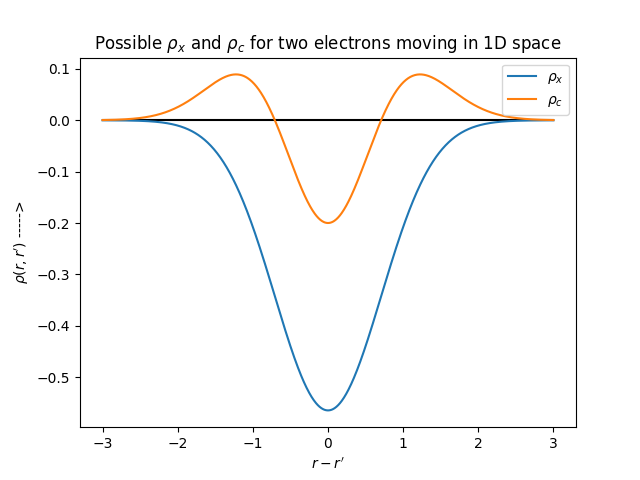
\includegraphics[scale=0.88]{nx_nc.png}
  \caption{Possible $\rho_x$ and $\rho_c$ for two $e^-$ moving in 1D line}
  \label{fig:XC-hole}
  \end{figure}
  We can observe from fig(\ref{fig:XC-hole}) and verify the properties derived in the above sections,
  \begin{enumerate}
  \item{The exchange hole is negative everywhere and is at maximum strength for the on-top value.}
  \item{The correlation hole is negative near the on-top region and positive for regions away from that $\rightarrow$ total integral is 0.}
  \item{Both the holes and hence the total hole also is strong for the on-top value but decays as $r_{12}$ increases.}
  \end{enumerate}
  Lets now look at the total hole arising due to the holes in fig(\ref{fig:XC-hole}),\\
  \begin{figure}[h]
  \centering
  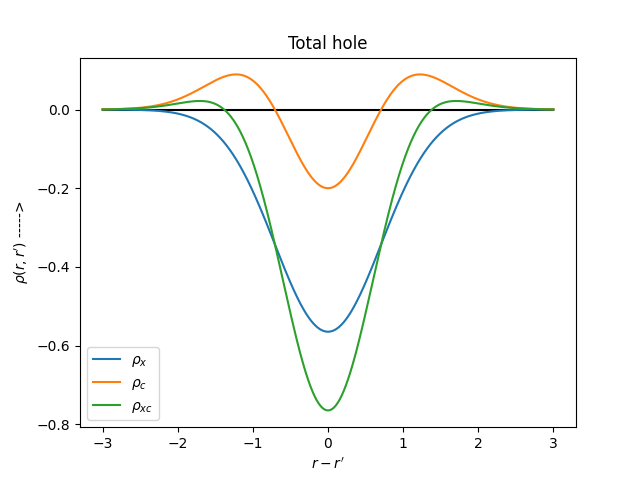
\includegraphics[scale=0.88]{nx_nc_ntotal.png}
  \caption{Total hole due to the X and C-holes in fig(\ref{fig:XC-hole})}
  \label{fig:total-hole}
  \end{figure}
  So we didn't realise it by looking at fig(\ref{fig:XC-hole}) that the X-hole and C-hole chosen were \textbf{wrong}. As we can see from fig(\ref{fig:total-hole}), the total hole would then be positive for some regions which clearly violates the negativity criterion (eqn(\ref{eq:27})). But there is a way around i.e if we can make slight modifications to any one (or either) of the holes, then we can make the total hole obey the sum-rule and other criteria also. This often occurs when the exchange and correlation part are taken from different models and such fuctionals should be cleverly handled so that the hole properties are not broken.
  
 \subsection*{\Large{So what criteria should be followed by model $E_{xc}$ ?}}
  As we saw from eqn(\ref{eq:23}), the $E_{xc}$ is the energy of interaction of an electron density with its hole. So the better we describe this (spherically averaged)exact-hole $\rightarrow$ the better will be our approximation to $E_{xc}$. To know whether our model hole is a good representation of the exact-hole we must know all the properties of the exact hole. BUT WE DON'T (till now). So for now, what we can actually tell is that, if our model-hole doesn't satisfy the properties derived in the previous sections (+some other known universal constraints\footnote{There are many known constraints like Leib-Oxford bound, Scaling properties etc. which must be followed along with what we derived.}) then it won't work for sure. 
  
 \subsection*{\Large{References}}
  \begin{enumerate}
	 \item{CECAM summer school(2017) video lectures by Levy,Perdew,Kieron Burke - \\ \underline{\url{https://www.youtube.com/channel/UCfLssAro7SMxgaeKTNFFeeA}}}
	 \item{ABC of DFT, Kieron Burke}
	 \item{A Chemist’s Guide to
Density Functional Theory, Wolfram Koch, Max C. Holthausen}
	 \item{Electronic Structure Calculations for Solids and Molecules- Theory and Computational Methods,Jorge Kohanoff}
	 \item{Modern Quantum Chemistry: Introduction to Advanced Electronic Structure, Attila Szabo , Neil S. Ostlund. }
	 \end{enumerate}
   \end{flushleft}
  \end{Large}    
  
\end{document}